\documentclass[a4paper]{article}
\usepackage[a4paper,margin=0mm]{geometry}
\usepackage{fontspec}
\usepackage{unicode-math}
\usepackage{tikz}
\usepackage[table]{xcolor}
\usepackage[absolute]{textpos}
\usepackage{enumitem}
\usepackage{array}
\usepackage{multirow}

\setmainfont{Libertinus Serif}
\setsansfont{Libertinus Sans}
\setmathfont{Libertinus Math}
\newfontfamily\trackedsans{Libertinus Sans}[LetterSpace=8.0]

\definecolor{accent}{HTML}{602785}
\definecolor{badge}{HTML}{B8A0C8}
\definecolor{ink}{HTML}{2A2E30}

\setlength{\TPHorizModule}{1mm}
\setlength{\TPVertModule}{1mm}
\setlength{\parindent}{0pt}
\pagestyle{empty}

\newcommand{\LCOL}{16mm}
\newcommand{\RCOL}{111mm}
\newcommand{\COLW}{83mm}

\newcommand{\topicheader}[2]{%
\begin{textblock*}{194mm}(16mm,10mm)
\begin{tikzpicture}
\node[fill=accent,text=white,font=\sffamily\bfseries\fontsize{13}{13}\selectfont,
      minimum width=9mm,minimum height=9mm,inner sep=0pt] at (4.5mm,-4.5mm) {#1};
\node[font=\sffamily\bfseries\fontsize{15}{16}\selectfont,text=ink,anchor=west] at (12mm,-4.5mm) {#2};
\end{tikzpicture}
\end{textblock*}
\begin{textblock*}{194mm}(16mm,22.5mm)

\begin{tikzpicture}
\fill[accent] (0,0) rectangle (194mm,0.5mm);
\end{tikzpicture}
\end{textblock*}
}

\newcommand{\pagefooter}[1]{%
\begin{textblock*}{194mm}(8mm,286.41mm)
  
\begin{tikzpicture}
    \fill[accent] (0,0) rectangle (194mm,0.6mm);
  \end{tikzpicture}
\end{textblock*}
\begin{textblock*}{63.59mm}(8mm,288.27mm)
  {\sffamily\bfseries\color{accent}\fontsize{13}{16}\selectfont SAT 1200+}
\end{textblock*}
\begin{textblock*}{10mm}(188mm,288.27mm)
  \centering{\sffamily\color{accent}\fontsize{14}{16}\selectfont #1}
\end{textblock*}
}

\newcommand{\colrule}[2]{%
\begin{textblock*}{1mm}(105mm,#1mm)
\begin{tikzpicture}
\draw[black!65,line width=0.5pt] (0,0) -- (0,#2mm);
\end{tikzpicture}
\end{textblock*}
}

\newcommand{\setkicker}[2]{%
{\sffamily\bfseries\fontsize{12}{14}\selectfont #1.}\ {\itshape\fontsize{11}{14}\selectfont\color{black!75} #2}\par\vspace{2mm}%
}

\setlength{\fboxsep}{1.4pt}
\setlength{\fboxrule}{0.5pt}
\newcommand{\pnum}[1]{\fcolorbox{ink}{white}{\sffamily\bfseries\fontsize{8}{8}\selectfont #1}~}

\newcommand{\qrbox}[1]{%
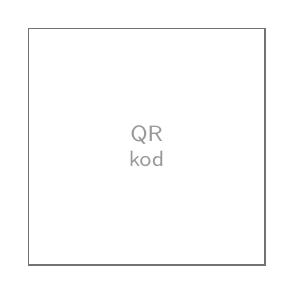
\begin{tikzpicture}
\draw[black!55,line width=0.6pt] (0,0) rectangle (30mm,30mm);
\node[black!40,font=\sffamily\fontsize{8}{9}\selectfont,align=center] at (15mm,15mm) {QR\\kod};
\end{tikzpicture}\\[1.5mm]
{\sffamily\fontsize{9}{11}\selectfont\color{black!70} #1}%
}

\arrayrulecolor{accent}
\setlength{\arrayrulewidth}{0.7pt}
\renewcommand{\arraystretch}{1.3}
\newcommand{\anstitle}[1]{{\sffamily\bfseries\color{accent}\fontsize{11}{13}\selectfont #1}\\[1.3mm]}

\begin{document}

% ================= PAGE 1: Set 1 | Set 2 =================
\topicheader{7}{Parabola Grafigi va Diskriminant}
\pagefooter{37}
\colrule{32}{238}
\mbox{}%

\begin{textblock*}{\COLW}(\LCOL,32mm)
{\fontsize{11.5}{14.5}\selectfont
\setkicker{1-to'plam}{Uchini, simmetriya o'qini, yo'nalishini va kengligini toping.}

\noindent\pnum{1} $y=3(x-1)^2+4$\\[20mm]
\noindent\pnum{2} $y=-2(x+3)^2-1$\\[20mm]
\noindent\pnum{3} $y=(x-5)^2+2$\\[20mm]
\noindent\pnum{4} $y=-\dfrac{1}{2}(x-2)^2+6$\\[20mm]
\noindent\pnum{5} $y=5(x+4)^2-7$\\[20mm]
\noindent\pnum{6} $y=-x^2+9$
}
\end{textblock*}

\begin{textblock*}{\COLW}(\RCOL,32mm)
{\fontsize{11.5}{14.5}\selectfont
\setkicker{2-to'plam}{$D=b^2-4ac$ ni hisoblang va yechimlar sonini ayting.}

\noindent\pnum{1} $x^2+5x+6=0$\\[20mm]
\noindent\pnum{2} $x^2-4x+4=0$\\[20mm]
\noindent\pnum{3} $x^2+2x+5=0$\\[20mm]
\noindent\pnum{4} $2x^2-3x-5=0$\\[20mm]
\noindent\pnum{5} $3x^2+2x+1=0$\\[20mm]
\noindent\pnum{6} $x^2-6x+9=0$
}
\end{textblock*}

\clearpage

% ================= PAGE 2: Set 3 | Set 4 =================
\topicheader{7}{Parabola Grafigi va Diskriminant}
\pagefooter{38}
\colrule{32}{238}
\mbox{}%

\begin{textblock*}{\COLW}(\LCOL,32mm)
{\fontsize{11.5}{14.5}\selectfont
\setkicker{3-to'plam}{$x$-kesmalarini (ildizlarni) toping.}

\noindent\pnum{1} $x^2-7x+10=0$\\[20mm]
\noindent\pnum{2} $x^2+x-12=0$\\[20mm]
\noindent\pnum{3} $2x^2-x-3=0$\\[20mm]
\noindent\pnum{4} $x^2-9=0$\\[20mm]
\noindent\pnum{5} $x^2+6x+9=0$\\[20mm]
\noindent\pnum{6} $3x^2+5x-2=0$
}
\end{textblock*}

\begin{textblock*}{\COLW}(\RCOL,32mm)
{\fontsize{11.5}{14.5}\selectfont
\setkicker{4-to'plam}{Uchini, diskriminantni va haqiqiy ildizlarni (bo'lsa) toping.}

\noindent\pnum{1} $y=x^2-4x+3$\\[27mm]
\noindent\pnum{2} $y=-x^2+4x-5$\\[27mm]
\noindent\pnum{3} $y=2x^2-8x+8$\\[27mm]
\noindent\pnum{4} $y=-3x^2+12x-9$\\[27mm]
\noindent\pnum{5} $y=x^2+2x+1$
}
\end{textblock*}

\clearpage

% ================= PAGE 3: Set 5 | Set 6 (spot the error) =================
\topicheader{7}{Parabola Grafigi va Diskriminant}
\pagefooter{39}
\colrule{32}{238}
\mbox{}%

\begin{textblock*}{\COLW}(\LCOL,32mm)
{\fontsize{11}{14}\selectfont
\setkicker{5-to'plam}{"$k$ ni toping" -- SAT uslubidagi diskriminant masalalari.}

\noindent\pnum{1} $x^2+kx+9=0$ tenglama aynan bitta haqiqiy yechimga ega bo'lishi uchun $k$ qanday qiymat(lar)ni qabul qilishi kerak?\\[14mm]
\noindent\pnum{2} $x^2-4x+k=0$ tenglama haqiqiy yechimga ega bo'lmasligi uchun $k$ qanday bo'lishi kerak?\\[14mm]
\noindent\pnum{3} $2x^2+4x+k=0$ tenglama ikkita haqiqiy yechimga ega bo'lishi uchun $k$ qanday bo'lishi kerak?\\[14mm]
\noindent\pnum{4} $x^2+6x+k=0$ tenglama aynan bitta haqiqiy yechimga ega bo'lishi uchun $k$ ni toping.\\[14mm]
\noindent\pnum{5} $kx^2+4x+4=0$ ($k\ne0$) tenglama haqiqiy yechimga ega bo'lmasligi uchun $k$ qanday bo'lishi kerak?
}
\end{textblock*}

\begin{textblock*}{\COLW}(\RCOL,32mm)
{\fontsize{10.5}{13.5}\selectfont
\setkicker{6-to'plam}{Xatoni toping -- buzilgan qadamni ayting, to'g'ri javobni bering.}

\noindent\pnum{1} $y=2(x-3)^2+5$ ifodasida ko'rsatilgan yechimda xato bor:\\[1mm]
\hspace*{7mm}\textit{``Uchi $(-3,5)$.''}\\[2mm]
\hspace*{7mm}Xato va to'g'ri javob: \makebox[52mm]{\dotfill}\\[8mm]

\noindent\pnum{2} $x^2+2x+5=0$ ifodasida ko'rsatilgan yechimda xato bor:\\[1mm]
\hspace*{7mm}\textit{``$D=4-20=-16$, demak 2 ta haqiqiy yechim bor, chunki D haqiqiy son.''}\\[2mm]
\hspace*{7mm}Xato va to'g'ri javob: \makebox[52mm]{\dotfill}\\[8mm]

\noindent\pnum{3} $y=-2x^2+8$ ifodasida ko'rsatilgan yechimda xato bor:\\[1mm]
\hspace*{7mm}\textit{``Yuqoriga ochiladi, chunki $x^2$ oldidagi son musbat 2.''}\\[2mm]
\hspace*{7mm}Xato va to'g'ri javob: \makebox[52mm]{\dotfill}\\[8mm]

\noindent\pnum{4} $x^2-5x+6=0$ ifodasida ko'rsatilgan yechimda xato bor:\\[1mm]
\hspace*{7mm}\textit{``$(x-2)(x-3)=0$, demak ildizlar $x=-2,-3$.''}\\[2mm]
\hspace*{7mm}Xato va to'g'ri javob: \makebox[52mm]{\dotfill}\\[8mm]

\noindent\pnum{5} $y=x^2-4x+4$ ifodasida ko'rsatilgan yechimda xato bor:\\[1mm]
\hspace*{7mm}\textit{``$D=16-16=0$, demak yechim yo'q.''}\\[2mm]
\hspace*{7mm}Xato va to'g'ri javob: \makebox[52mm]{\dotfill}
}
\end{textblock*}

\clearpage

% ================= PAGE 4: Set 7 (bonus) =================
\topicheader{7}{Parabola Grafigi va Diskriminant}
\pagefooter{40}
\colrule{32}{238}
\mbox{}%

\begin{textblock*}{\COLW}(\LCOL,32mm)
{\fontsize{11}{14}\selectfont
\setkicker{7-to'plam}{Bonus / qiyin -- har biriga taxminan 90 soniya.}

\noindent\pnum{1} To'pning balandligi $h(t)=-16t^2+64t+5$ formulasi bilan ifodalanadi. U qaysi vaqtda eng baland nuqtaga yetadi va bu balandlik qanchaga teng?\\[14mm]
\noindent\pnum{2} $y=x^2+(k+2)x+9$ grafigi $x$ o'qiga aynan bitta nuqtada tegishi uchun $k$ ning qiymatini toping.\\[14mm]
\noindent\pnum{3} Parabolaning uchi $(2,-3)$ nuqtada va u $(0,5)$ nuqtadan o'tadi. $y=ax^2+bx+c$ dagi $a$, $b$, $c$ ni toping.\\[16mm]
\noindent\pnum{4} $3x^2-2x+1=0$ tenglama nechta haqiqiy yechimga ega -- uning grafigi $x$ o'qini kesib o'tadimi, tegadimi yoki umuman tegmaydimi?\\[14mm]
\noindent\pnum{5} Agar $x^2+bx+16=0$ tenglamaning diskriminanti $0$ ga teng bo'lsa, $b$ ning barcha mumkin qiymatlarini toping.
}
\end{textblock*}

\clearpage

% ================= PAGE 5: Javoblar part 1 (Sets 1-4) =================
\topicheader{7}{Parabola Grafigi va Diskriminant}
\pagefooter{41}
\mbox{}%

\begin{textblock*}{194mm}(16mm,30mm)
{\bfseries\itshape\color{accent}\fontsize{19}{21}\selectfont\centering Javoblar\par}
\end{textblock*}

\begin{textblock*}{194mm}(16mm,44mm)
{\fontsize{9.5}{12}\selectfont
\centering
\renewcommand{\arraystretch}{1.25}
\begin{tabular}{|>{\centering\arraybackslash}p{20mm}|>{\centering\arraybackslash}p{8mm}|p{144mm}|}
\hline
\rowcolor{badge!55}\textbf{To'plam} & \textbf{\#} & \textbf{Javob}\\
\hline
\multirow{6}{20mm}{\centering 1-to'plam} & 1 & Uchi $(1,4)$, o'q $x=1$, yuqoriga ochiladi, torroq\\\cline{2-3}
 & 2 & Uchi $(-3,-1)$, o'q $x=-3$, pastga ochiladi, torroq\\\cline{2-3}
 & 3 & Uchi $(5,2)$, o'q $x=5$, yuqoriga ochiladi, $y=x^2$ bilan bir xil kenglikda\\\cline{2-3}
 & 4 & Uchi $(2,6)$, o'q $x=2$, pastga ochiladi, kengroq\\\cline{2-3}
 & 5 & Uchi $(-4,-7)$, o'q $x=-4$, yuqoriga ochiladi, torroq\\\cline{2-3}
 & 6 & Uchi $(0,9)$, o'q $x=0$, pastga ochiladi, $y=x^2$ bilan bir xil kenglikda\\\hline
\multirow{3}{20mm}{\centering 2-to'plam} & 1--2 & 1) $D=1$, 2 yechim \quad 2) $D=0$, 1 yechim\\\cline{2-3}
 & 3--4 & 3) $D=-16$, 0 yechim \quad 4) $D=49$, 2 yechim\\\cline{2-3}
 & 5--6 & 5) $D=-8$, 0 yechim \quad 6) $D=0$, 1 yechim\\\hline
\multirow{3}{20mm}{\centering 3-to'plam} & 1--2 & 1) $x=2,5$ \quad 2) $x=-4,3$\\\cline{2-3}
 & 3--4 & 3) $x=-1,\frac32$ \quad 4) $x=-3,3$\\\cline{2-3}
 & 5--6 & 5) $x=-3$ (qo'sh ildiz) \quad 6) $x=-2,\frac13$\\\hline
\multirow{5}{20mm}{\centering 4-to'plam} & 1 & Uchi $(2,-1)$, $D=4$, ildizlar $x=1,3$\\\cline{2-3}
 & 2 & Uchi $(2,-1)$, $D=-4$, haqiqiy ildiz yo'q\\\cline{2-3}
 & 3 & Uchi $(2,0)$, $D=0$, ildiz $x=2$\\\cline{2-3}
 & 4 & Uchi $(2,3)$, $D=36$, ildizlar $x=1,3$\\\cline{2-3}
 & 5 & Uchi $(-1,0)$, $D=0$, ildiz $x=-1$\\\hline
\end{tabular}
}
\end{textblock*}

\clearpage

% ================= PAGE 6: Javoblar part 2 (Sets 5-7) + QR =================
\topicheader{7}{Parabola Grafigi va Diskriminant}
\pagefooter{42}
\mbox{}%

\begin{textblock*}{194mm}(16mm,30mm)
{\fontsize{9.5}{12}\selectfont
\centering
\renewcommand{\arraystretch}{1.25}
\begin{tabular}{|>{\centering\arraybackslash}p{20mm}|>{\centering\arraybackslash}p{8mm}|p{144mm}|}
\hline
\rowcolor{badge!55}\textbf{To'plam} & \textbf{\#} & \textbf{Javob}\\
\hline
\multirow{3}{20mm}{\centering 5-to'plam} & 1--2 & 1) $k=\pm6$ \quad 2) $k>4$\\\cline{2-3}
 & 3--4 & 3) $k<2$ \quad 4) $k=9$\\\cline{2-3}
 & 5 & 5) $k>1$\\\hline
\multirow{5}{20mm}{\centering 6-to'plam} & 1 & Xato -- vertex shakli $a(x-h)^2+k$, demak uchi $(h,k)=(3,5)$, $(-3,5)$ emas.\\\cline{2-3}
 & 2 & Xato -- $D<0$ bo'lsa yechim \textbf{yo'q}, "D haqiqiy son" emas, D ning ishorasi muhim.\\\cline{2-3}
 & 3 & Xato -- oldidagi manfiy ishora e'tiborga olinmagan: $a=-2<0$, demak pastga ochiladi.\\\cline{2-3}
 & 4 & Xato -- $(x-2)=0$ dan $x=2$ chiqadi, $x=-2$ emas. To'g'ri ildizlar: $x=2,3$.\\\cline{2-3}
 & 5 & Xato -- $D=0$ bo'lsa aynan \textbf{bitta} yechim bor (parabola $x$ o'qiga tegadi), yechim yo'q emas.\\\hline
\multirow{5}{20mm}{\centering 7-to'plam} & 1 & $t=2$ soniya, eng baland nuqta $=69$\\\cline{2-3}
 & 2 & $k=4$ yoki $k=-8$\\\cline{2-3}
 & 3 & $a=2$, $b=-8$, $c=5$\\\cline{2-3}
 & 4 & $D=-8<0$ -- 0 ta haqiqiy yechim, grafik $x$ o'qini kesib o'tmaydi va tegmaydi ham\\\cline{2-3}
 & 5 & $b=\pm8$\\\hline
\end{tabular}
}
\end{textblock*}

\begin{textblock*}{194mm}(16mm,230mm)
\centering
{\sffamily\fontsize{9.5}{11.5}\selectfont\color{black!70} Video yechimlar va qo'shimcha testlar uchun quyidagi QR kodlarni skanerlang:}\\[4mm]
\begin{minipage}[t]{32mm}\centering\qrbox{YouTube}\end{minipage}%
\hspace{16mm}%
\begin{minipage}[t]{32mm}\centering\qrbox{Telegram}\end{minipage}
\end{textblock*}

\end{document}
